\documentclass[11pt]{article}
\usepackage{lastpage}
\usepackage[hmargin=2cm, top=2.7cm, bottom=3.5cm, footskip=0.5cm]{geometry}
\usepackage{hyperref}
\usepackage{url}
\usepackage{float}
\usepackage{parskip}
\usepackage[citestyle=authoryear-comp,natbib=true]{biblatex}
\usepackage{pdflscape}
\usepackage[absolute]{textpos}
\usepackage{rotating} %for xtable sideways
\usepackage{verbatim}
\usepackage{longtable}
\usepackage{lipsum}
\usepackage[acronym,nomain]{glossaries}
\usepackage{fancyhdr, graphicx, lastpage, ifthen, lscape}
\usepackage[table]{xcolor}

\bibliography{bibliography.bib}


% For knitr
\usepackage{lmodern}
\usepackage{amssymb,amsmath}
\usepackage{ifxetex,ifluatex}
\usepackage{fixltx2e} % provides \textsubscript
\ifnum 0\ifxetex 1\fi\ifluatex 1\fi=0 % if pdftex
  \usepackage[T1]{fontenc}
  \usepackage[utf8]{inputenc}
\else % if luatex or xelatex
  \ifxetex
    \usepackage{mathspec}
    \usepackage{xltxtra,xunicode}
  \else
    \usepackage{fontspec}
  \fi
  \defaultfontfeatures{Mapping=tex-text,Scale=MatchLowercase}
  \newcommand{\euro}{€}
\fi
% use upquote if available, for straight quotes in verbatim environments
\IfFileExists{upquote.sty}{\usepackage{upquote}}{}
% use microtype if available
\IfFileExists{microtype.sty}{%
\usepackage{microtype}
\UseMicrotypeSet[protrusion]{basicmath} % disable protrusion for tt fonts
}{}
\usepackage{color}
\usepackage{fancyvrb}
\newcommand{\VerbBar}{|}
\newcommand{\B}{\rule[-2ex]{0pt}{0pt}} % bottom strut
\newcommand{\VERB}{\Verb[commandchars=\\\{\}]}
\DefineVerbatimEnvironment{Highlighting}{Verbatim}{commandchars=\\\{\}}
% Add ',fontsize=\small' for more characters per line
\usepackage{framed}
\definecolor{shadecolor}{RGB}{248,248,248}
\newenvironment{Shaded}{\begin{snugshade}}{\end{snugshade}}
\newcommand{\KeywordTok}[1]{\textcolor[rgb]{0.13,0.29,0.53}{\textbf{{#1}}}}
\newcommand{\DataTypeTok}[1]{\textcolor[rgb]{0.13,0.29,0.53}{{#1}}}
\newcommand{\DecValTok}[1]{\textcolor[rgb]{0.00,0.00,0.81}{{#1}}}
\newcommand{\BaseNTok}[1]{\textcolor[rgb]{0.00,0.00,0.81}{{#1}}}
\newcommand{\FloatTok}[1]{\textcolor[rgb]{0.00,0.00,0.81}{{#1}}}
\newcommand{\CharTok}[1]{\textcolor[rgb]{0.31,0.60,0.02}{{#1}}}
\newcommand{\StringTok}[1]{\textcolor[rgb]{0.31,0.60,0.02}{{#1}}}
\newcommand{\CommentTok}[1]{\textcolor[rgb]{0.56,0.35,0.01}{\textit{{#1}}}}
\newcommand{\OtherTok}[1]{\textcolor[rgb]{0.56,0.35,0.01}{{#1}}}
\newcommand{\AlertTok}[1]{\textcolor[rgb]{0.94,0.16,0.16}{{#1}}}
\newcommand{\FunctionTok}[1]{\textcolor[rgb]{0.00,0.00,0.00}{{#1}}}
\newcommand{\RegionMarkerTok}[1]{{#1}}
\newcommand{\ErrorTok}[1]{\textbf{{#1}}}
\newcommand{\NormalTok}[1]{{#1}}
\providecommand{\tightlist}{%
   \setlength{\itemsep}{0pt}\setlength{\parskip}{0pt}}
\makeatletter
\def\maxwidth{\ifdim\Gin@nat@width>\linewidth\linewidth\else\Gin@nat@width\fi}
\def\maxheight{\ifdim\Gin@nat@height>\textheight\textheight\else\Gin@nat@height\fi}
% End For knitr

\renewcommand{\abstractname}{Overview}


% Configure hyperref formatting bookmarks and references
\hypersetup{
  colorlinks = true, % color links instead of covering them w/red boxes
  urlcolor   = blue, % color for external hyperlinks
  linkcolor  = cyan, % color of internal links
  citecolor  = gray  % color of citations
}


%this is to adjust header and footer in landscaped pages
\fancypagestyle{lscape}{%
    \fancyhf{} % clear all header and footer fields
    \fancyhead[R]{\begin{footnotesize}
    \begin{textblock}{1}(0.7,1.5){\color{gray}\rotatebox{90}{Short Title}}\end{textblock}
    \end{footnotesize} }
    \fancyfoot[L]{\begin{footnotesize}
    \begin{textblock}{1}(21,1.75){\color{gray}\rotatebox{90}{Page \thepage{}~of~\pageref{LastPage}}}\end{textblock}
    \end{footnotesize} }
    \fancyfoot[R]{\begin{footnotesize}
%     \begin{textblock}{19.8}[-0.01,{\DynLength}](1.5,23.20){\color{gray}\rotatebox{90}{\Rver}}\end{textblock}
    \begin{textblock}{19.8}(1.5,23.20){\color{gray}\rotatebox{90}{\Rver}}\end{textblock}
    \end{footnotesize} }
    \setlength{\TPHorizModule}{1cm}
    \setlength{\TPVertModule}{1cm}
    \renewcommand{\headrulewidth}{0.0pt}
    \renewcommand{\footrulewidth}{0.0pt}}

%set header and footer for first page
\renewcommand{\headrulewidth}{0.8pt}
\renewcommand{\footrulewidth}{0.8pt}
\fancyhead[L]{
\includegraphics[height=0.8cm]{./logos/scharp.png}}
\fancyhead[C]{
\includegraphics[height=0.8cm]{./logos/new_VISC_logo_color.jpg}}
\fancyhead[R]{
\includegraphics[height=0.8cm]{./logos/FredHutch_h_tag_4col_CMYK_tm.png}}
\fancyfoot[C]{Page \thepage{}~of~\pageref{LastPage}}

%decrease margins for landscape pages
\newenvironment{changemargin}[2]{%
\begin{list}{}{%
\setlength{\topsep}{0pt}%
\setlength{\leftmargin}{#1}%
\setlength{\rightmargin}{#2}%
%\setlength{\listparindent}{\parindent}%
%\setlength{\itemindent}{\parindent}%
\setlength{\parsep}{\parskip}%
}%
\item[]}{\end{list}}

%page settings
\setlength{\footskip}{56pt}
\pagestyle{fancy}
\setlength{\parindent}{0pt}
\makeglossaries
\begin{document}


%get current date into insertdate
\makeatletter
\let\insertdate\@date
\makeatother

%begin To and From Section
\makeatletter
\newcommand\tabfill[1]{%
  \dimen@\linewidth
  \advance\dimen@\@totalleftmargin
  \advance\dimen@-\dimen\@curtab
  \parbox[t]\dimen@{%
    \leftskip=2em\hspace*{-2em}#1\ifhmode\strut\fi}%
}
\makeatother

\vspace{0.1cm}
\begin{flushleft}
\begin{tabbing}
this line is to\= set up the tab stop \kill
{\bf Date:} \> \insertdate\\
{\bf To:} \>  \tabfill{FirstNameA LastNameA, FirstNameB LastNameB, FirstNameC LastNameC, FirstNameD LastNameD, FirstNameE LastNameE, FirstNameF LastNameF}\\
{\bf From:} \> \tabfill{FirstNameA LastNameA, FirstNameB LastNameB}\\
{\bf RE:} \> \tabfill{Title of Your Submission}\\
{\bf cc:} \> \tabfill{FirstNameA LastNameA, FirstNameB LastNameB, FirstNameC LastNameC, FirstNameD LastNameD, FirstNameE LastNameE}\\
{\bf Contact:} \> \tabfill{FirstNameA LastNameA, \href{mailto:foo@bar.com}{\nolinkurl{foo@bar.com}}  }\\
\end{tabbing}
\end{flushleft}

\hrule

\vspace{2cm}

%begin contents section

%change color of header and footer text to gray
\makeatletter
\patchcmd{\@fancyhead}{\rlap}{\color{gray}\rlap}{}{}
\patchcmd{\headrule}{\hrule}{\color{gray}\hrule}{}{}
\patchcmd{\@fancyfoot}{\rlap}{\color{gray}\rlap}{}{}
\patchcmd{\footrule}{\hrule}{\color{gray}\hrule}{}{}
\makeatother



\begin{abstract}
A short summary about your report.
\end{abstract}

\newpage
\fancyhead[R]{\em Short Title}
\fancyhead[C]{}
\fancyhead[L]{\em VISC report}

\printglossaries

\section{Summary of Main Results}\label{summary-of-main-results}

Summary Here

\section{Background}\label{background}

Backgroup Text Here

\section{Objectives}\label{objectives}

Objectives Here

\section{Endpoints}\label{endpoints}

Endpoints Here

\section{Lab Methods}\label{lab-methods}

Lab Methods Here

\section{Statistical Methods}\label{statistical-methods}

Statistical Methods Here

\section{Participant Cohort}\label{participant-cohort}

Participant Cohort

\section{Results}\label{results}

Writing up results section

\subsection{Section 1}\label{section-1}

\subsection{Section 2}\label{section-2}

Testing Reference: Huang and Gottardo (2013).

\section{Figures and Tables}\label{figures-and-tables}

\clearpage

\begin{figure}[htbp]
\centering
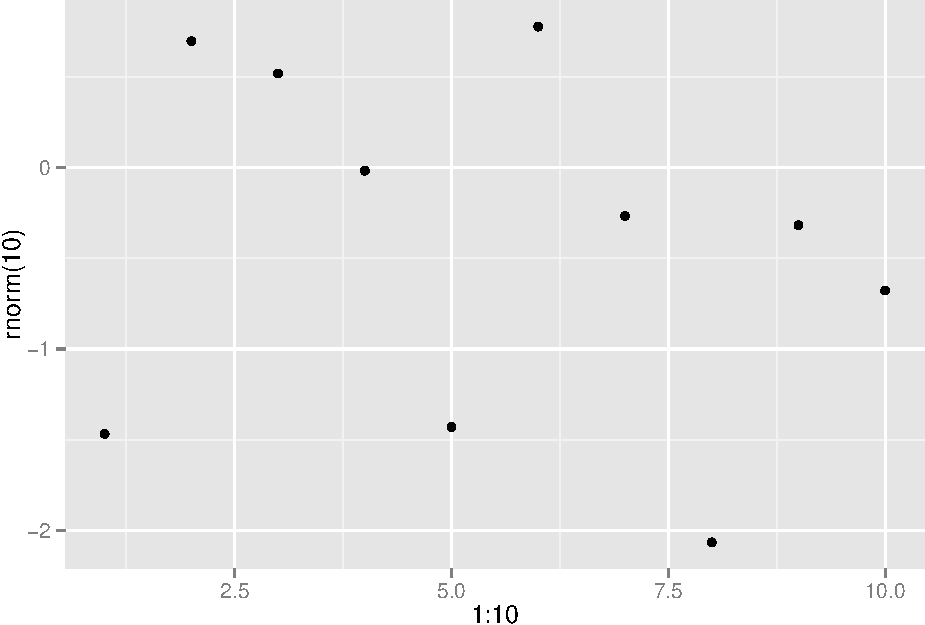
\includegraphics{skeleton_files/figure-latex/unnamed-chunk-5-1.pdf}
\caption{A simple figure}
\end{figure}

\begin{table}

\caption{A simple table}
\centering
\begin{tabular}[t]{l|r|r|r|r|r|r|r|r|r|r|r}
\hline
  & mpg & cyl & disp & hp & drat & wt & qsec & vs & am & gear & carb\\
\hline
Mazda RX4 & 21.0 & 6 & 160.0 & 110 & 3.90 & 2.620 & 16.46 & 0 & 1 & 4 & 4\\
\hline
Mazda RX4 Wag & 21.0 & 6 & 160.0 & 110 & 3.90 & 2.875 & 17.02 & 0 & 1 & 4 & 4\\
\hline
Datsun 710 & 22.8 & 4 & 108.0 & 93 & 3.85 & 2.320 & 18.61 & 1 & 1 & 4 & 1\\
\hline
Hornet 4 Drive & 21.4 & 6 & 258.0 & 110 & 3.08 & 3.215 & 19.44 & 1 & 0 & 3 & 1\\
\hline
Hornet Sportabout & 18.7 & 8 & 360.0 & 175 & 3.15 & 3.440 & 17.02 & 0 & 0 & 3 & 2\\
\hline
Valiant & 18.1 & 6 & 225.0 & 105 & 2.76 & 3.460 & 20.22 & 1 & 0 & 3 & 1\\
\hline
Duster 360 & 14.3 & 8 & 360.0 & 245 & 3.21 & 3.570 & 15.84 & 0 & 0 & 3 & 4\\
\hline
Merc 240D & 24.4 & 4 & 146.7 & 62 & 3.69 & 3.190 & 20.00 & 1 & 0 & 4 & 2\\
\hline
Merc 230 & 22.8 & 4 & 140.8 & 95 & 3.92 & 3.150 & 22.90 & 1 & 0 & 4 & 2\\
\hline
Merc 280 & 19.2 & 6 & 167.6 & 123 & 3.92 & 3.440 & 18.30 & 1 & 0 & 4 & 4\\
\hline
Merc 280C & 17.8 & 6 & 167.6 & 123 & 3.92 & 3.440 & 18.90 & 1 & 0 & 4 & 4\\
\hline
Merc 450SE & 16.4 & 8 & 275.8 & 180 & 3.07 & 4.070 & 17.40 & 0 & 0 & 3 & 3\\
\hline
Merc 450SL & 17.3 & 8 & 275.8 & 180 & 3.07 & 3.730 & 17.60 & 0 & 0 & 3 & 3\\
\hline
Merc 450SLC & 15.2 & 8 & 275.8 & 180 & 3.07 & 3.780 & 18.00 & 0 & 0 & 3 & 3\\
\hline
Cadillac Fleetwood & 10.4 & 8 & 472.0 & 205 & 2.93 & 5.250 & 17.98 & 0 & 0 & 3 & 4\\
\hline
Lincoln Continental & 10.4 & 8 & 460.0 & 215 & 3.00 & 5.424 & 17.82 & 0 & 0 & 3 & 4\\
\hline
Chrysler Imperial & 14.7 & 8 & 440.0 & 230 & 3.23 & 5.345 & 17.42 & 0 & 0 & 3 & 4\\
\hline
Fiat 128 & 32.4 & 4 & 78.7 & 66 & 4.08 & 2.200 & 19.47 & 1 & 1 & 4 & 1\\
\hline
Honda Civic & 30.4 & 4 & 75.7 & 52 & 4.93 & 1.615 & 18.52 & 1 & 1 & 4 & 2\\
\hline
Toyota Corolla & 33.9 & 4 & 71.1 & 65 & 4.22 & 1.835 & 19.90 & 1 & 1 & 4 & 1\\
\hline
Toyota Corona & 21.5 & 4 & 120.1 & 97 & 3.70 & 2.465 & 20.01 & 1 & 0 & 3 & 1\\
\hline
Dodge Challenger & 15.5 & 8 & 318.0 & 150 & 2.76 & 3.520 & 16.87 & 0 & 0 & 3 & 2\\
\hline
AMC Javelin & 15.2 & 8 & 304.0 & 150 & 3.15 & 3.435 & 17.30 & 0 & 0 & 3 & 2\\
\hline
Camaro Z28 & 13.3 & 8 & 350.0 & 245 & 3.73 & 3.840 & 15.41 & 0 & 0 & 3 & 4\\
\hline
Pontiac Firebird & 19.2 & 8 & 400.0 & 175 & 3.08 & 3.845 & 17.05 & 0 & 0 & 3 & 2\\
\hline
Fiat X1-9 & 27.3 & 4 & 79.0 & 66 & 4.08 & 1.935 & 18.90 & 1 & 1 & 4 & 1\\
\hline
Porsche 914-2 & 26.0 & 4 & 120.3 & 91 & 4.43 & 2.140 & 16.70 & 0 & 1 & 5 & 2\\
\hline
Lotus Europa & 30.4 & 4 & 95.1 & 113 & 3.77 & 1.513 & 16.90 & 1 & 1 & 5 & 2\\
\hline
Ford Pantera L & 15.8 & 8 & 351.0 & 264 & 4.22 & 3.170 & 14.50 & 0 & 1 & 5 & 4\\
\hline
Ferrari Dino & 19.7 & 6 & 145.0 & 175 & 3.62 & 2.770 & 15.50 & 0 & 1 & 5 & 6\\
\hline
Maserati Bora & 15.0 & 8 & 301.0 & 335 & 3.54 & 3.570 & 14.60 & 0 & 1 & 5 & 8\\
\hline
Volvo 142E & 21.4 & 4 & 121.0 & 109 & 4.11 & 2.780 & 18.60 & 1 & 1 & 4 & 2\\
\hline
\end{tabular}
\end{table}

\clearpage 

\begin{table}[ht]
\centering
{\footnotesize
\begin{tabular}{ll}
  \hline
  \hline
version & R version 3.2.1 (2015-06-18) \\ 
  system & x86\_64, linux-gnu \\ 
  ui & X11 \\ 
  language & (EN) \\ 
  collate & en\_US.UTF-8 \\ 
  tz &  \\ 
  repo & https://github.fhcrc.org/VIDD-VISC/scharpTemplates.git \\ 
  location & inst/rmarkdown/templates/visc\_report/skeleton \\ 
  file name & skeleton.Rmd \\ 
   \hline
\end{tabular}
}
\caption{Supplemental Table: Reproducibility Software Session Information} 
\label{session_info}
\end{table}\begin{table}[ht]
\centering
{\footnotesize
\begin{tabular}{llll}
  \hline
package & version & date & source \\ 
  \hline
data.table & 1.9.7 & 2016-04-29 & Github (Rdatatable/data.table@5c5067d) \\ 
  devtools & 1.8.0 & 2015-05-09 & CRAN (R 3.2.1) \\ 
  ggplot2 & 2.1.0 & 2016-05-02 & Github (hadley/ggplot2@59c503b) \\ 
  knitr & 1.12.3 & 2016-01-22 & CRAN (R 3.2.1) \\ 
  reshape2 & 1.4.1 & 2014-12-06 & CRAN (R 3.2.1) \\ 
  xtable & 1.7-4 & 2014-09-12 & CRAN (R 3.2.1) \\ 
   \hline
\end{tabular}
}
\caption{Supplemental Table: Reproducibility Software Package Version Information} 
\label{session_info2}
\end{table}

\clearpage 

\section*{References}\label{references}
\addcontentsline{toc}{section}{References}

Huang, Yunda, and Rapha{ë}l Gottardo. 2013. ``Comparability and
reproducibility of biomedical data.'' \emph{Briefings in Bioinformatics}
14 (4): 391--401.
\label{LastPageOfBackMatter}~
\end{document}


